\documentclass[11pt]{article}
\usepackage[utf8]{inputenc} % Para caracteres en espa�ol
\usepackage{amsmath,amsthm,amsfonts,amssymb,amscd}
\usepackage{multirow,booktabs}
\usepackage[table]{xcolor}
\usepackage{fullpage}
\usepackage{lastpage}
\usepackage{enumitem}
\usepackage{multicol}
\usepackage{fancyhdr}
\usepackage{mathrsfs}
\usepackage{wrapfig}
\usepackage{setspace}
\usepackage{esvect}
\usepackage{calc}
\usepackage{multicol}
\usepackage{cancel}
\usepackage{graphicx}
\graphicspath{ {pictures/} }
\usepackage[retainorgcmds]{IEEEtrantools}
\usepackage[margin=3cm]{geometry}
\usepackage{amsmath}
\newlength{\tabcont}
\setlength{\parindent}{0.0in}
\setlength{\parskip}{0.05in}
\usepackage{empheq}
\usepackage{framed}
\usepackage{newtxmath}
\usepackage{euscript}
\DeclareMathAlphabet{\mathpzc}{T1}{pzc}{m}{it}
\usepackage[most]{tcolorbox}
\usepackage{xcolor}
\colorlet{shadecolor}{orange!15}
\parindent 0in
\parskip 12pt
\geometry{margin=1in, headsep=0.25in}
\theoremstyle{definition}
\newtheorem{defn}{Definition}
\newtheorem{reg}{Rule}
\newtheorem{exer}{Exercise}
\newtheorem{note}{Note}
\newcommand{\volume}{{\ooalign{\hfil$V$\hfil\cr\kern0.08em--\hfil\cr}}}
\newcommand{\parr}{\mathbin{\|}} % Parralel Symbol
\begin{document}
\setcounter{section}{4} %Section before the section you want. I want section 1 I put 0
\setcounter{page}{8} %page number you want to be the first page
\setcounter{equation}{16} %equation before the equation you want I want equation 2 I put 1
%\definecolor{babyblue}{rgb}{0.54, 0.81, 0.94}
\definecolor{babyblueeyes}{rgb}{0.63, 0.79, 0.95}
\definecolor{babyblue}{rgb}{0.69, 0.88, 0.9}

 \pagestyle{fancy}
 
\fancyhf{}
\rhead{Section 5:  Collisions}
\rfoot{Page \thepage}
\thispagestyle{empty}


\begin{center}
{\LARGE \bf Section 5:  Collisions}\\
{\large AE435}\\
Spring 2018
\end{center}

\vspace{5mm}
\section{Atom-Atom Collisions}
\vspace{25mm}
\tableofcontents
\newpage
\subsection{Elastic}
Lennard-Jones "6-12" potential profile used for elastic scattering, it combines:
\begin{itemize}
\item Weak dipole attraction,  r-6
\item Short-range "hard-core" repulsion,  r-12
\end{itemize}
 
   \begin{center}
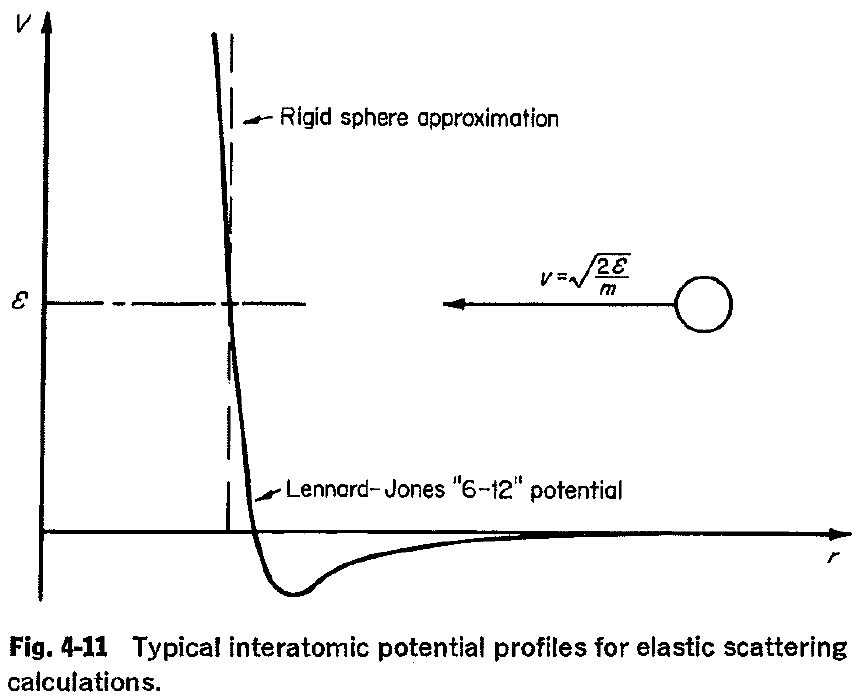
\includegraphics[scale=.7]{12.png}
\end{center}

The repulsion results from interactions between bound electrons as the two atoms attempt to interpenetrate.
Neutral elastic collision are studied in great detail (both experimentally and theoretically) because of their importance in determining transport properties

\newpage
\subsection{Inelastic}

Mean atomic speeds are so small compared to mean electron speeds, these are generally not important in EP plasmas.
\end{document}